\documentclass{article}
%==============================================================================%
%	                          Packages                                     %
%==============================================================================%
% Packages
\usepackage[utf8]{inputenc}
\usepackage{graphicx}
\usepackage{float}
\usepackage{amsmath}
\usepackage{amssymb}
\usepackage{braket}
\usepackage{subcaption}
\usepackage[margin=0.7in]{geometry}
\usepackage[version=4]{mhchem}
%==============================================================================%
%                           User-Defined Commands                              %
%==============================================================================%
% User-Defined Commands
\newcommand{\be}{\begin{equation}}
\newcommand{\ee}{\end{equation}}
\newcommand{\benum}{\begin{enumerate}}
\newcommand{\eenum}{\end{enumerate}}
\newcommand{\pd}{\partial}
\newcommand{\dg}{\dagger}
\newcommand{\sumzero}{\sum_{n=0}^\infty}
\newcommand{\sumone}{\sum_{n=1}^\infty}
%==============================================================================%
%                             Title Information                                %
%==============================================================================%
\title{Chem237: Lecture 11}
\date{4/10/18}
\author{Alan Robledo}
%==============================================================================%
%	Everyone Please Make Comments if Something Needs to be Reviewed        %
%                           Or just fix it yourself!                           %
%==============================================================================%
\begin{document}
\maketitle
%==============================================================================%
% The end of integral transforms lecture should go here.
%==============================================================================%
\section*{Linear Algebra}
Just as we've seen with a Fourier Series, some topics can be better understood when we think about it in terms of Linear Algebra.
Therefore, we will dive right into the topic just as our Math Methods book does in Chapter 6.

These next few lectures should not be seen as the equivalent of taking your first Linear Algebra course because such a course handles a topic as abstract as this one very carefully by making sure every definition is given and then proven.
In mathematical methods, we will find ourselves using ideas that have been proven rigorously by mathematicians and simply treating these ideas as if it is all well known information.
With that said, we will run through all the well known information first and then see how all of this information can be used to obtain solutions to problems of interest.

\subsection*{Vectors and Vector Spaces}
In every standard calculus course you are told about objects known as vectors.
And you learn that a vector is a mathematical object that is defined by its direction and length.
So in 2 dimensions, you can have a whole space of vectors which could look something like this,
\begin{figure}[H]
  \centering
  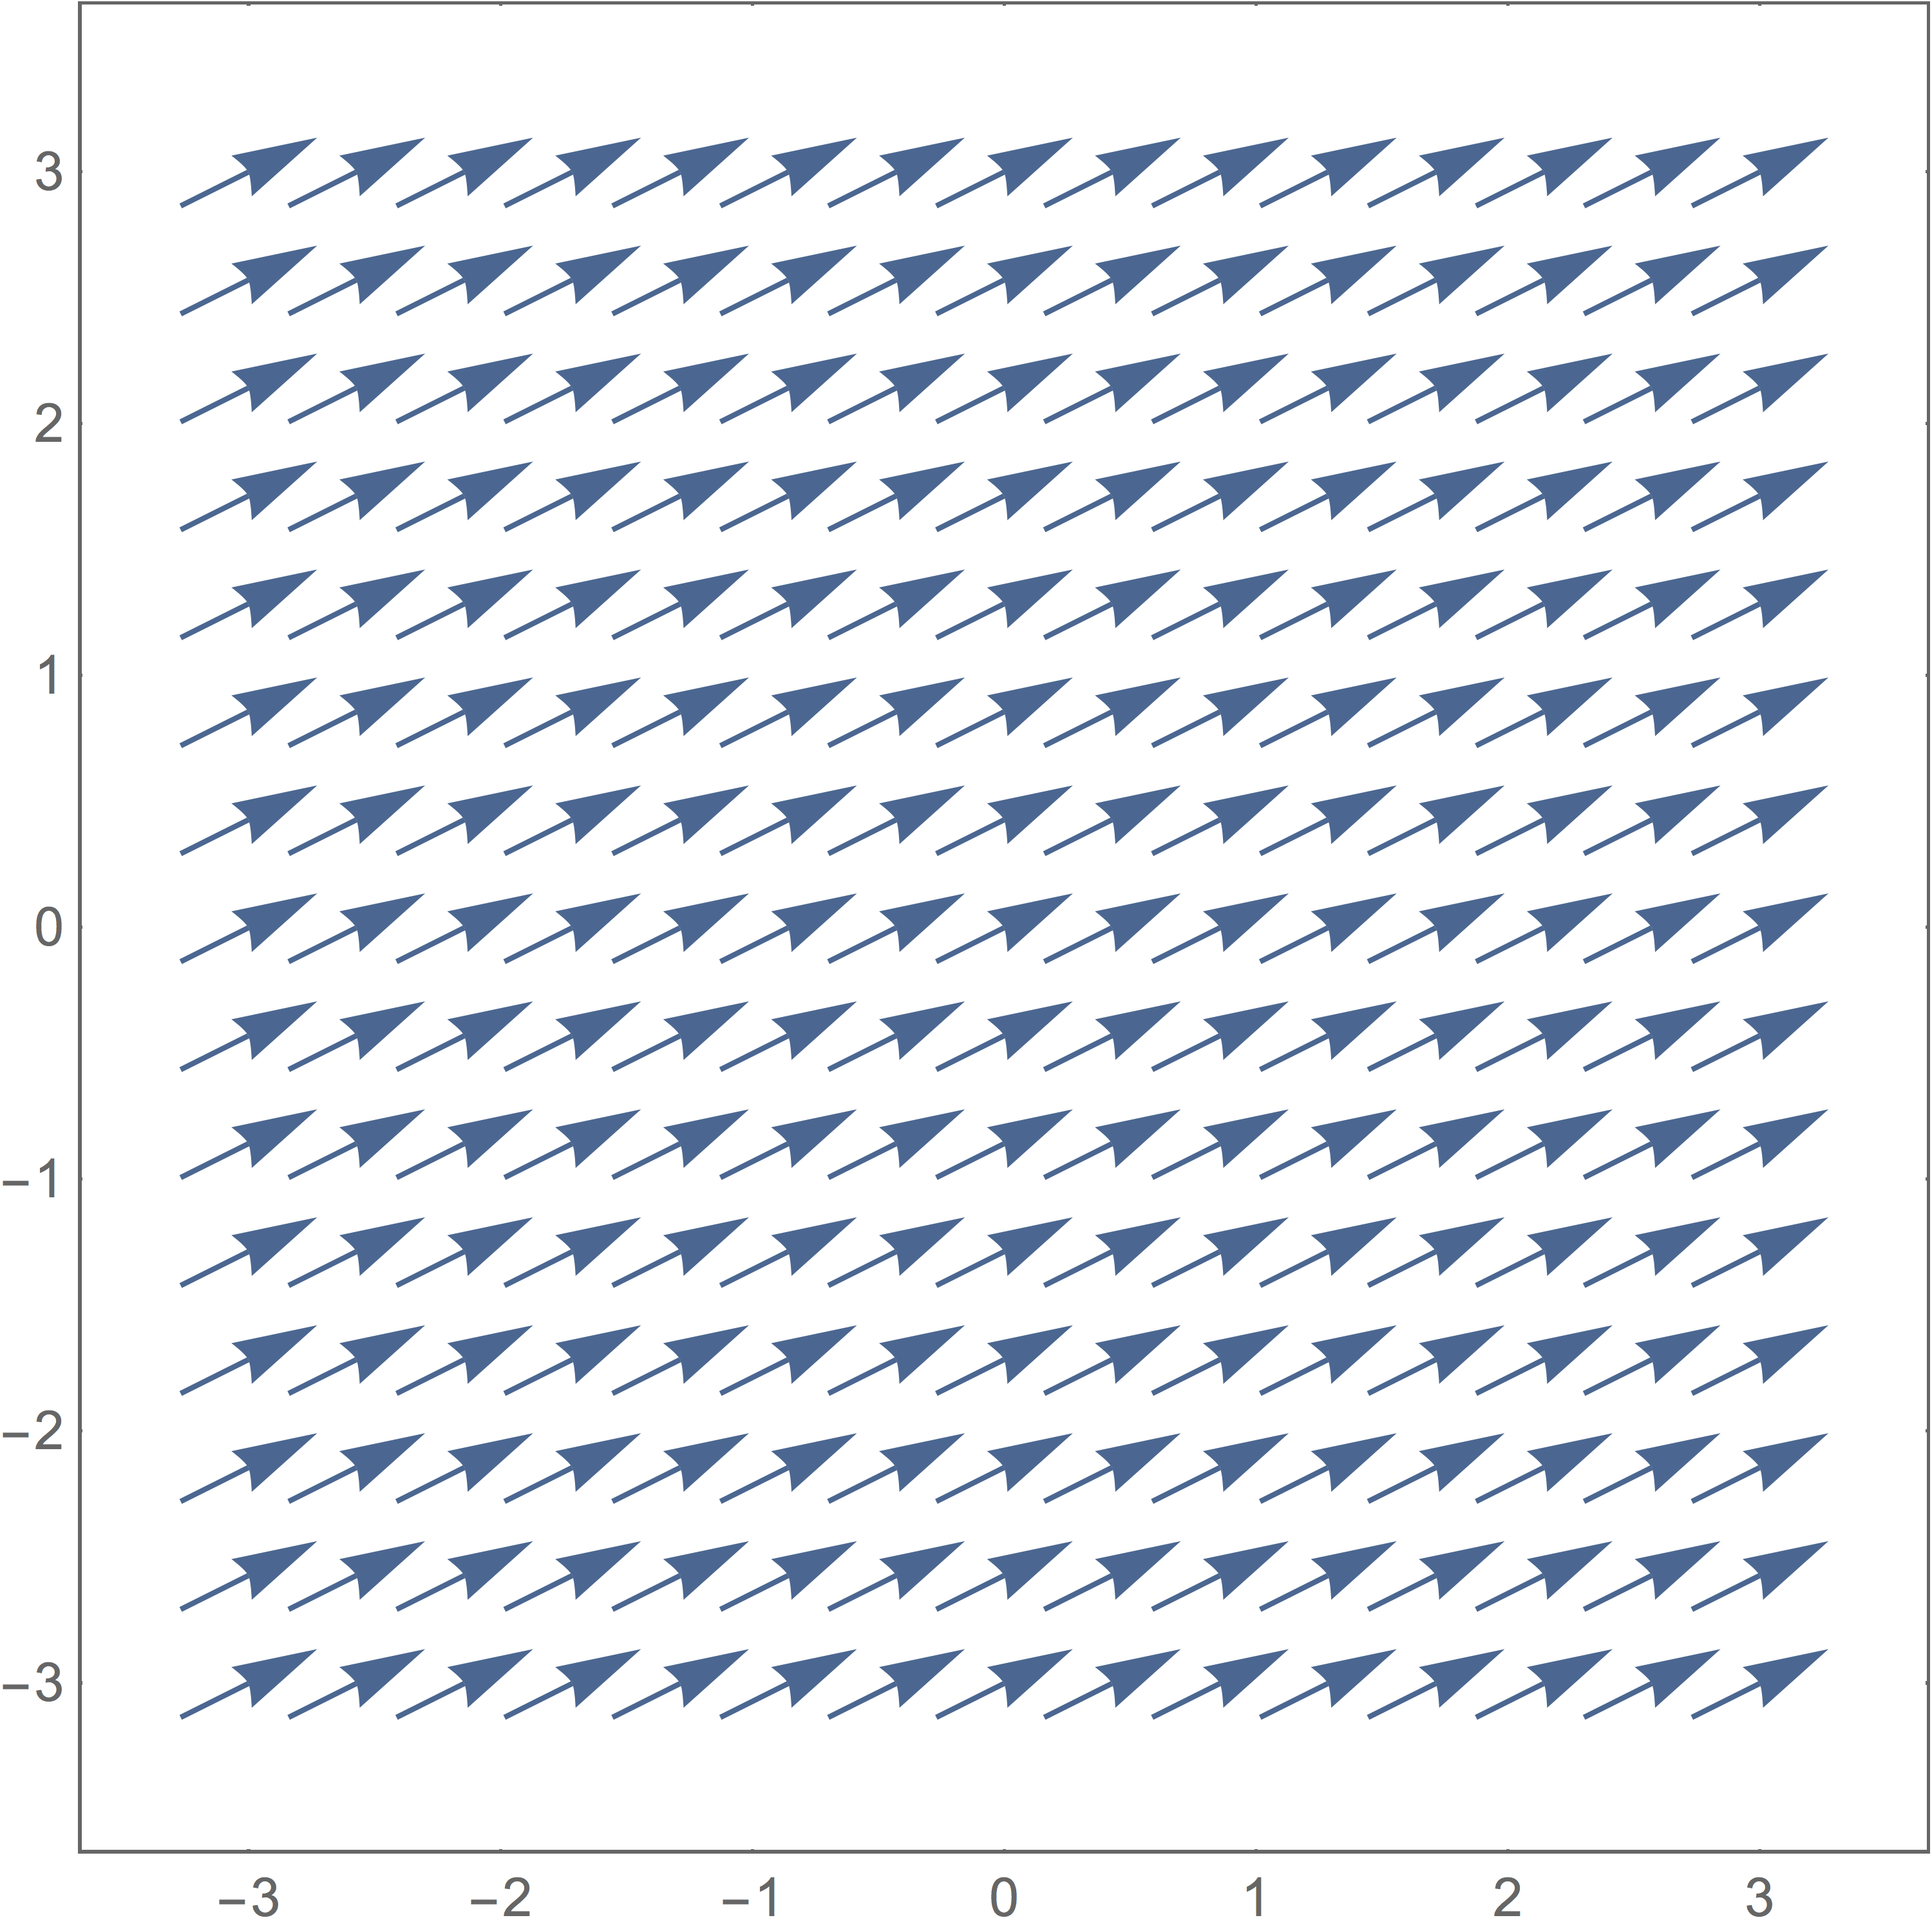
\includegraphics[scale=0.7]{Figures/vectors.png}
    \caption{An example of a constant vector field $\vec{F}(x,y) = 2 \hat{i} + \hat{j}$.}
  \label{fig:rotation}
\end{figure}
\noindent
and we call this set of objects (vectors) a linear vector space.

Each vector space is said to be closed under addition and multiplication.
In other words, for every vector $\vec{u}$ and $\vec{v}$ there exists another vector $\vec{u} + \vec{v}$, and for every scalar a and vector $\vec{u}$ there exists a vector $a \vec{u}$.
This means that vectors maintain properties such as the
\be
  \begin{split}
    \text{Commutative property:} \quad & \vec{u} + \vec{v} = \vec{v} + \vec{u} \\
    \text{Associative property:} \quad & (\vec{u} + \vec{v}) + \vec{r} = \vec{u} + (\vec{v} + \vec{r}) \\
    \text{Distributive scalar property:} \quad & a(\vec{u} + \vec{v}) = a\vec{u} + a\vec{v} \\
    \text{Distributive vector property:} \quad & (a + b)\vec{u} = a\vec{u} + b\vec{u} \\
  \end{split}
\ee
We also always assume that for any vector $\vec{u}$ there exists a null vector $\vec{0}$ such that
\be
  \vec{u} + \vec{0} = \vec{u}
\ee
and an additive inverse vector $-\vec{u}$ such that
\be
  \vec{u} + (- \vec{u}) = \vec{u} - \vec{u} = \vec{0}
\ee
These are some of the main properties of vector spaces that are important to know for solving problems that require the use of vectors.
While figure 1 shows how we can represent vectors pictorally, we can represent vectors numerically as a set of numbers
\be
  \vec{u} = < u_1 , u_2 , \hdots , u_n >
\ee
where n is the dimension of the vector space in question.
These can be thought of as the coordinates of a vector.
Some people use ( \quad ) instead of $<$ $>$ when writing vectors but either is acceptable, regardless of what anyone says.
Just be consistent.

A vector can also be defined as either a column vector
\[
\vec{u} =
\begin{bmatrix}
  u_{1} \\
  \vdots \\
  u_{n} \\
\end{bmatrix}
\]
or a row vector
\[
\vec{u} =
\begin{bmatrix}
  u_{1} & \cdots & u_{n} \\
\end{bmatrix}
\]

When we have a vector's coordinates, we can find out the length of the vector by finding its magnitude.
Notation-wise, the length of a vector $\vec{u}$ is denoted as $| \vec{u} |$ and this length is often reffered to as just u, which is the name of the vector without the arrow over it.
We can also define $| \vec{u} |$ as the norm of a vector $\vec{u}$, which is commonly given by the definition of the L2-norm
\be
  | \vec{u} | = \sqrt{u^2_1 + u^2_2 + \hdots + u^2_n}
\ee

In order to assign a value to a vector's length, we have to impose a \textbf{coordinate system/axes} and make use of the concept of \textbf{projection}.
This concept was explained briefly in lecture 8 when we discussed Fourier Series/Transform.

Before we go into this, we should first talk about linear operators that operate on vectors, aka matrices.
\subsection*{Matrices}
If we think of vectors as an array of numbers with size $n$, then matrices can be thought of as an array of arrays with size MxN, where M denotes the number of rows and N denotes the number of columns.
So a matrix A of size MxN would be written as:
\[
\textbf{A} =
\begin{bmatrix}
  A_{11} & \cdots & A_{1N} \\
  \vdots & & \vdots \\
  A_{M1} & \cdots & A_{MN}
\end{bmatrix}
\]

Matrices aren't meant to be visualized the way vectors are.
But matrices have properties that are important to know which are similar to vectors such as the
\be
  \begin{split}
    \text{Commutative property:} \quad & \textbf{A} + \textbf{B} = \textbf{B} + \textbf{A} \\
    \text{Associative property:} \quad & (\textbf{A} + \textbf{B}) + \textbf{C} = \textbf{A} + (\textbf{B} + \textbf{C} \\
    \text{Distributive scalar property:} \quad & a(\textbf{A} + \textbf{B}) = a\textbf{A} + a\textbf{B} \\
    \text{Distributive matrix property:} \quad & (a + b)\textbf{A} = a\textbf{A} + b\textbf{A} \\
  \end{split}
\ee

If we had two matrices \textbf{A} and \textbf{B} such that $\textbf{A} \in \mathbb{C}^{MxN}$ and $\textbf{B} \in \mathbb{C}^{NxK}$ we could define the multiplication of the two matrices as
\be \label{eq:matmul}
  \textbf{A} \textbf{B} = \textbf{C}
\ee
where \textbf{C} is a matrix such that $\textbf{C} \in \mathbb{C}^{MxK}$.
Therefore, the only way for the multiplication to work is if the number of columns of the left matrix is equal to the number of rows of the right matrix.
A useful way to write the multiplication is with summation notation,
\be \label{eq:matmul_sum}
  \sum\limits_{n=1}^{N} A_{mn} B_{nk} = C_{mk}
\ee
where n is summed over all possible values of m and k.
Notice how we used lowercase letters for m and k because we are saying that m can take on values from 1 $\hdots$ M and k can take on values from 1 $\hdots$ K.
Equation \ref{eq:matmul_sum} is more preffered when you're working out a problem and need to keep track of your variables, especially when you are coding the multiplication of two matrices.
Therefore, it might help to see what is actually going on in with the sum.
Equation \ref{eq:matmul_sum} says that
\be
  A_{m1} B_{1k} + A_{m2} B_{2k} + \hdots A_{m(N-1)} B_{(N-1)k} + A_{mN} B_{Nk} = C_{mk}
\ee
which means that for one element of the matrix C say the mk element, we need to single out the mth row of matrix A and the kth column of matrix B, multiply the corresponding entries together, and then add up the products.

\[
\begin{bmatrix}
  \vdots & \vdots & & \vdots & \vdots \\
  A_{m1} & A_{m2} & \cdots & A_{m(N-1)} & A{mN} \\
  \vdots & \vdots & & \vdots & \vdots \\
\end{bmatrix}
\begin{bmatrix}
  & \cdots & B_{1k} & \cdots & \\
  & \cdots & B_{2k} & \cdots & \\
  & & \vdots & & \\
  & \cdots & B_{(N-1)k} & \cdots & \\
  & \cdots & B_{Nk} & \cdots &
\end{bmatrix}
=
\begin{bmatrix}
   & \cdots & \\
  \vdots & C_{mk} & \vdots \\
   & \cdots & \\
\end{bmatrix}
\]

We can also multiply matrices with vectors and the summation would look very similar.
If we had the same matrix \textbf{A} with an M-dimensional vector $\vec{u}$, their multiplication would give a new vector $\vec{v}$
\be
  v_{m} = \sum_{n=1}^{N} A_{mn} u_{n}
\ee
Notice that the equation above tells us that we could find the mth coordinate of our new vector by taking the mth row of \textbf{A} and multiplying the corresponding values with the coordinates of $\vec{u}$.
When you're dealing with multiple sums, the work can get pretty messy, so it useful to use \textbf{einstein notation}.
%==============================================================================%
% We don't go over einstein notation but it might be useful to add a tiny section about it.
%==============================================================================%

Back to matrix properties, there exists a matrix \textbf{I} called a unit matrix or identity matrix such that for any matrix \textbf{A}
\be
  \textbf{I} \textbf{A} = \textbf{A} \textbf{I} = \textbf{A}
\ee
which is often thought of as multiplying by one for matrices.
Therefore, the identity matrix is a diagonal matrix of ones
\be
\begin{bmatrix}
   1 & 0\\
   0 & 1
\end{bmatrix}
,
\begin{bmatrix}
   1 & 0 & 0\\
   0 & 1 & 0\\
   0 & 0 & 1
\end{bmatrix}
, \dots
\ee
There also exists a matrix \textbf{0} called the null matrix such that each element of the matrix is zero.
Therefore,
\be
  \textbf{A} \textbf{0} = \textbf{0} \textbf{A} = \textbf{0} \quad \text{and} \quad \textbf{A} + \textbf{0} = \textbf{A}
\ee

A common mistake that people make is thinking of multiplying matrices the same way as multiplying scalars.
If you have two matrices \textbf{A} and \textbf{B} such that
\be
  \textbf{A} \textbf{B} = \textbf{C}
\ee
then you could solve for \textbf{B} by left multiplying both sides of the equation by the inverse of \textbf{A}
\be
  \textbf{A}^{-1} \textbf{A} \textbf{B} = \textbf{A}^{-1} \textbf{C} \quad \Rightarrow \quad \textbf{B} = \textbf{A}^{-1} \textbf{C}
\ee
because of the property $\textbf{A} \textbf{A}^{-1} = \textbf{A}^{-1} \textbf{A} = \textbf{I}$ and because the concept of dividing by matrices does not exist.
Similarly, we could solve for \textbf{A} by right multiplying by the inverse of \textbf{B}
\be
  \textbf{A} \textbf{B} \textbf{B}^{-1} = \textbf{C} \textbf{B}^{-1} \quad \Rightarrow \quad \textbf{A} = \textbf{C} \textbf{B}^{-1}
\ee
Using these tools, we can discuss the concept of a matrix being associated with a linear transformation.
\subsection*{Linear Transformation}
A linear transformation \textit{T} is when we create a mapping from one vector space to another using a matrix, i.e.\\
$\textit{T}: \mathbb{C}^N \rightarrow \mathbb{C}^M$.
Applying the transformation is as easy as multiplying any two matrices, because that's exactly what it is.

For example, consider two vector spaces in $\mathbb{R}^2$.
We can take any vector and rotate it counterclockwise by some degree $\theta$ by using the rotation matrix \textbf{R}$_{\theta}$
\begin{equation}
  \textbf{R}_{\theta} =
  \begin{bmatrix}
    \cos{\theta} & -\sin{\theta}\\
    \sin{\theta} & \cos{\theta} \\
  \end{bmatrix}
\end{equation}
If we wanted to visualize this, consider a vector $\vec{v}_1 = \begin{bmatrix} 1 \\ 0 \end{bmatrix}$.
We can rotate the vector 45 degrees = $\frac{\pi}{4}$ radians by multiplying it with the rotation matrix \textbf{R}$_\frac{\pi}{4}$
\begin{equation}
  \textbf{R}_\frac{\pi}{4} \vec{v}_1 =
  \begin{bmatrix}
    \cos{( \frac{\pi}{4} )} & -\sin{( \frac{\pi}{4} )}\\[6pt]
    \sin{( \frac{\pi}{4} )} & \cos{( \frac{\pi}{4} )} \\
  \end{bmatrix}
  \begin{bmatrix}
    1 \\ 0
  \end{bmatrix}
  =
  \begin{bmatrix}
    \frac{1}{\sqrt{2}} \\[6pt] \frac{1}{\sqrt{2}}
  \end{bmatrix}
  = \vec{v}_2
\end{equation}
and we can verify that the rotation was successful with a plot of $\vec{v}_1$ and $\vec{v}_2$.
\begin{figure}[H]
  \centering
  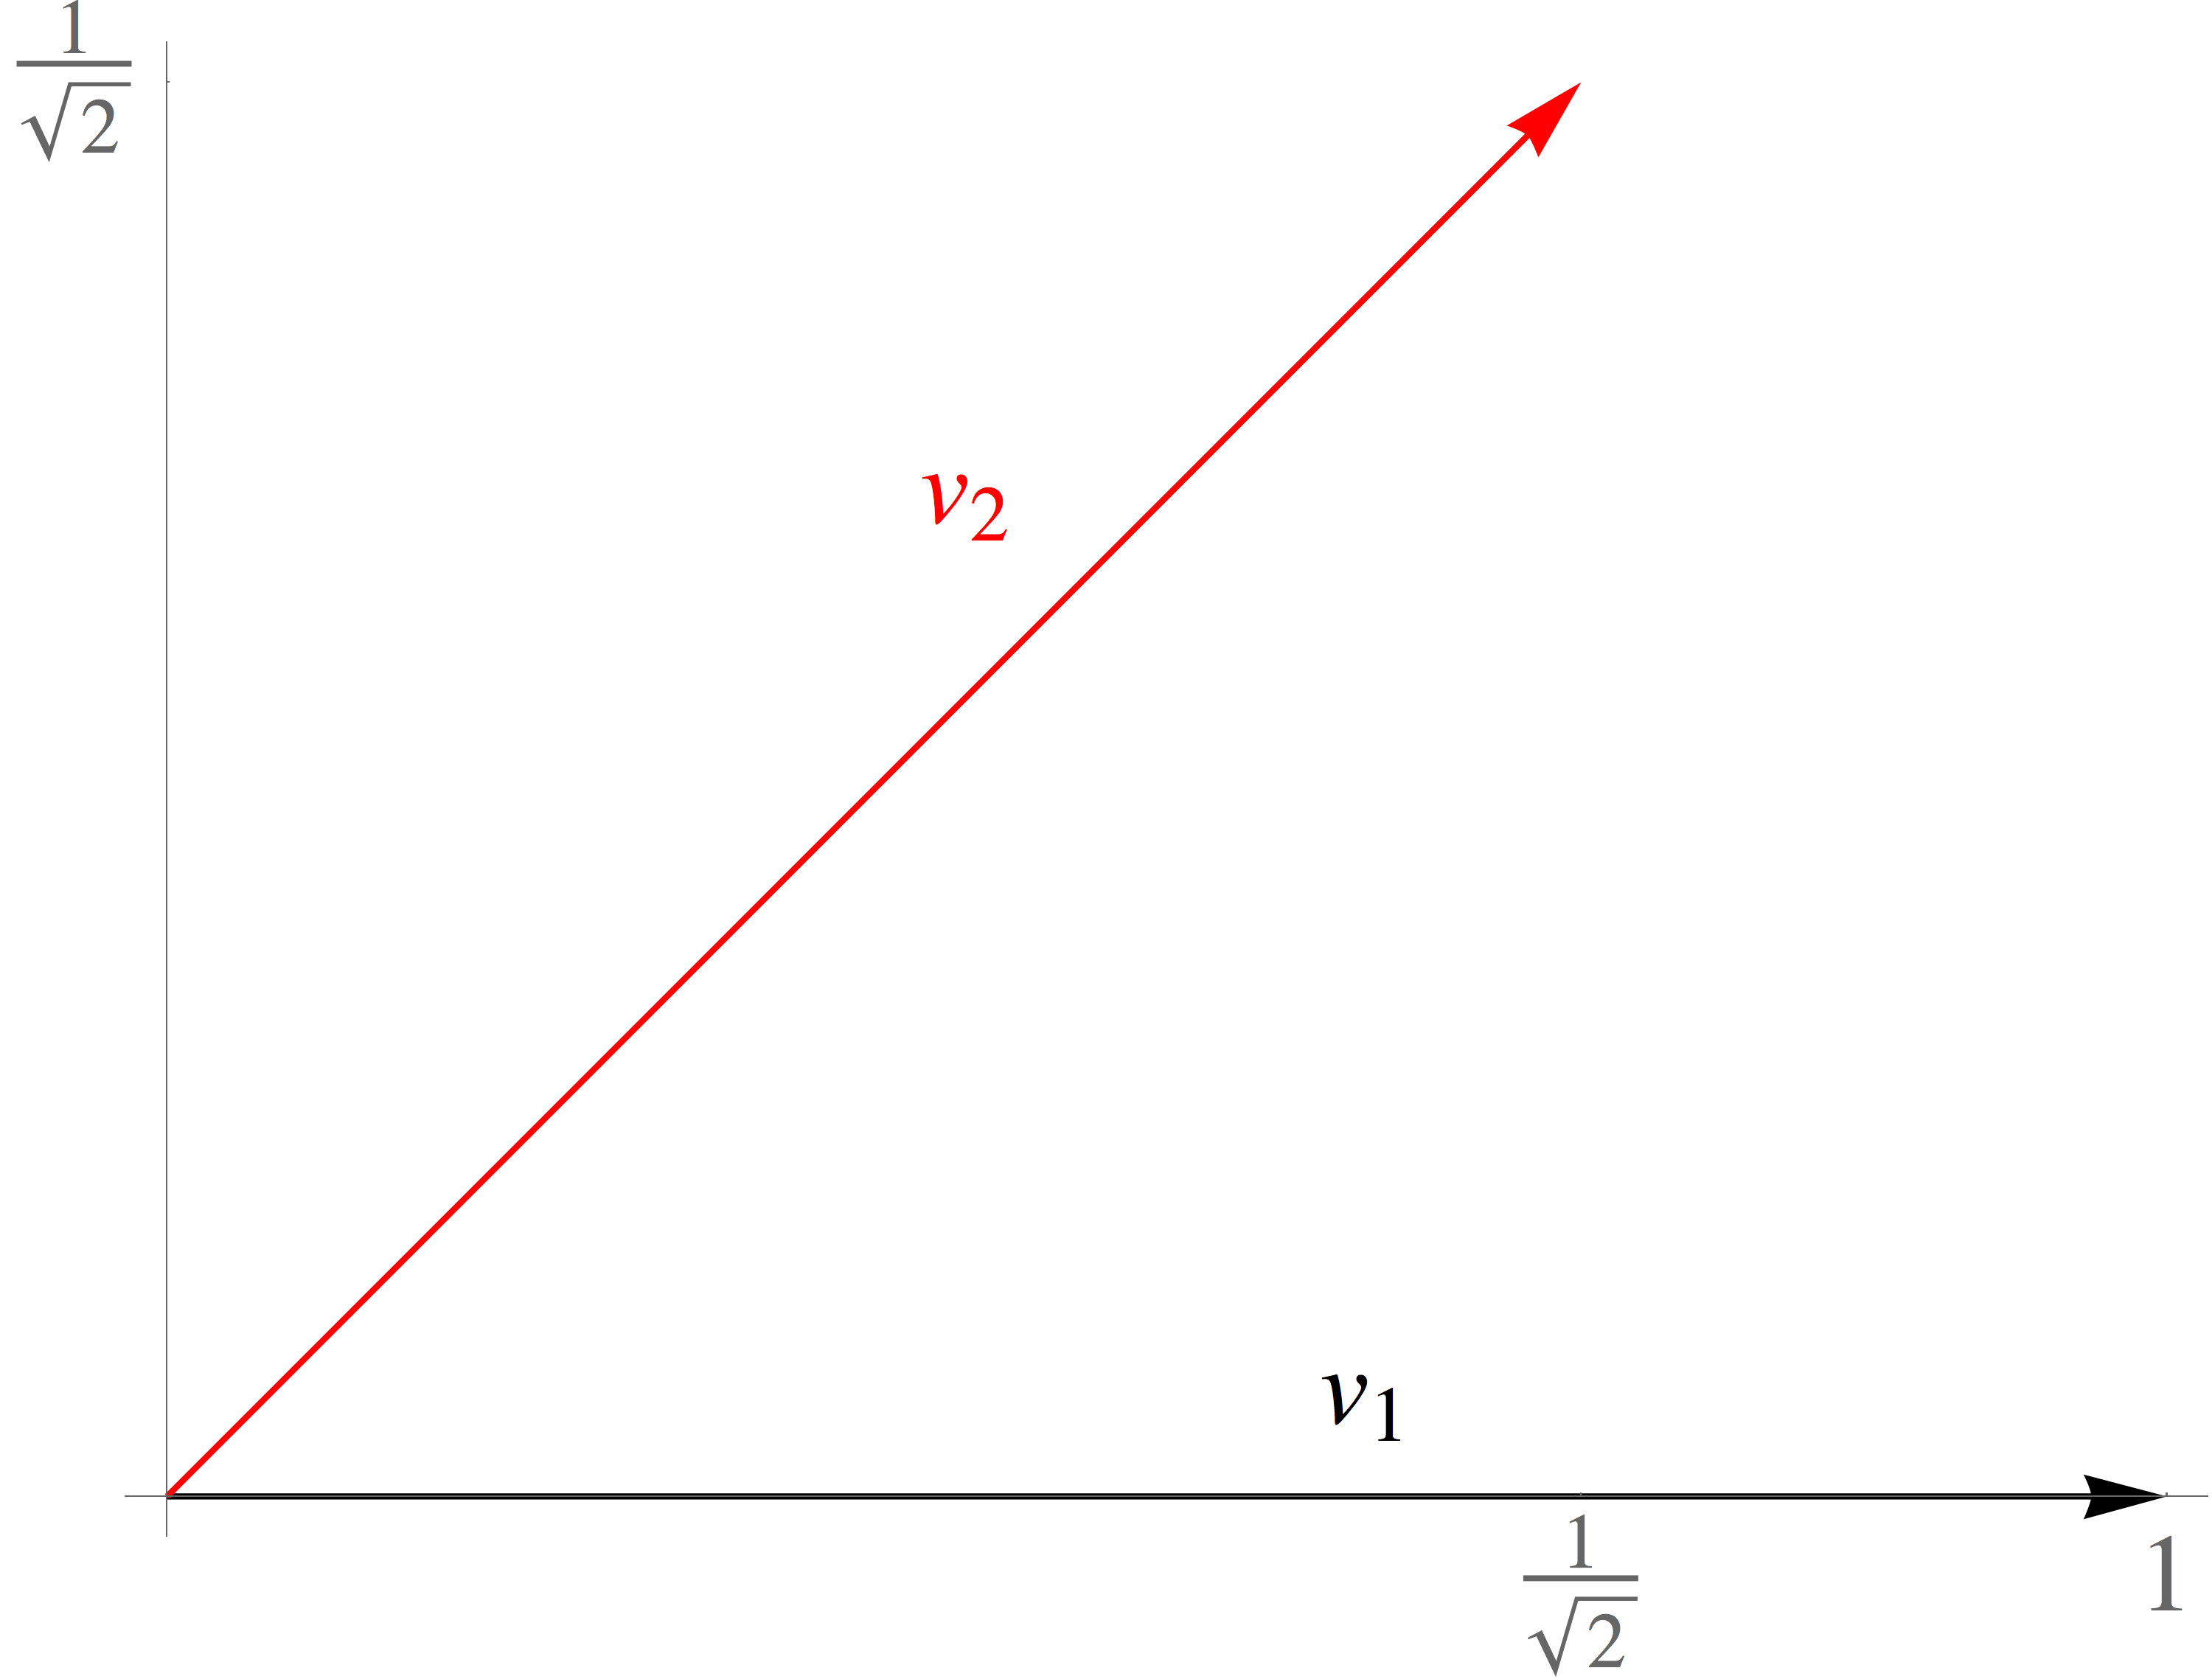
\includegraphics[scale=0.7]{Figures/rotation.png}
    \caption{$\vec{v}_1 = \begin{bmatrix} 1 \\ 0 \end{bmatrix}$ being rotated 45 degrees counterclockwise to produce $\vec{v}_2$ using the rotation matrix.}
  \label{fig:rotation}
\end{figure}
The rotation matrix is a special matrix because it has the following properties:
\begin{enumerate}
  \item \textbf{R}$_{\theta}$\textbf{R}$_{\theta'}$ = \textbf{R}$_{\theta'}$\textbf{R}$_{\theta}$
  \item \textbf{R}$_{\theta}$\textbf{R}$_{\theta'}$ = \textbf{R}$_{\theta + \theta'}$
  \item \textbf{R}$_{\theta}$\textbf{R}$_{-\theta}$ = \textbf{R}$_{0}$ = \textbf{I}
  \item \textbf{R}$_{\theta}^T$ = \textbf{R}$_{\theta}^{-1}$
\end{enumerate}
and property number 4 is why we call the rotation matrix an \textbf{orthognal matrix}.
The left hand side of property 4 is called the transpose matrix.
Transposing a matrix means taking the columns of a matrix and turning them into rows.
For example,
\begin{equation}
  \textbf{R}_{\theta}^{T} =
  \begin{bmatrix}
    \cos{\theta} & \sin{\theta}\\
    -\sin{\theta} & \cos{\theta} \\
  \end{bmatrix}.
\end{equation}
So in general, for any matrix \textbf{A},
\begin{equation}
  A_{mn}^T = A_{nm} .
\end{equation}

Finding the inverse of the matrix is more difficult.
In some cases, the inverse of a matrix may not exist.
To determine the existence of an inverse, it would be easier to first compute the determinant of the matrix, which we will discuss next lecture.

\end{document}
